\section{Motivație}

Anual se produc peste 8 000 de accidente rutiere grave în România, din care rezultă peste 7 000 de răniți grav și peste 2 000 de persoane decedate. Principalul motiv al tuturor acestor incidente, este de departe reprezentat de erorile umane, de la neatenție sau lipsa de experiență până la oboseală.
\begin{figure}[!h]
	\centering
	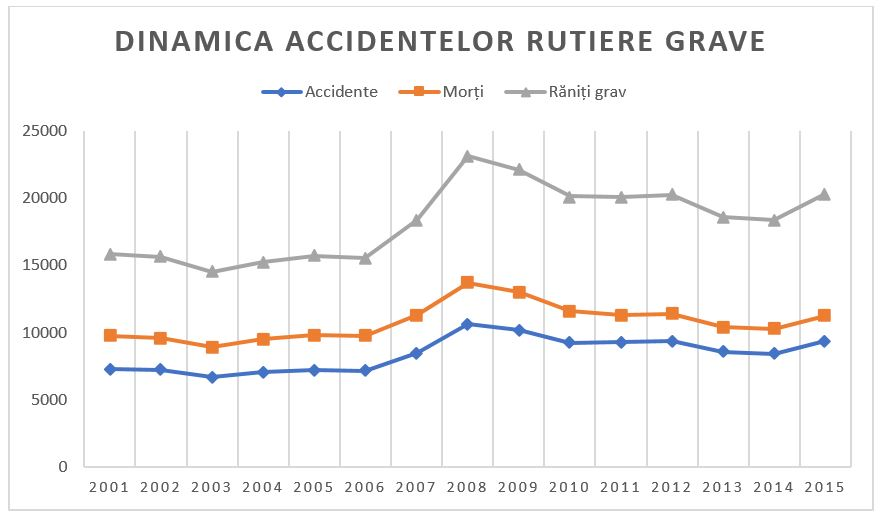
\includegraphics[max width=15cm,max height=15cm,keepaspectratio]{img_1_1}
	\caption{Dinamica accidentelor grave produse în România în perioada 2001 - 2015.}
\end{figure} 

Însă o foarte mare parte a erorilor ce duc la producerea de accidente pot fi evitate cu ajutorul unor sisteme dotate cu inteligență artificială. Sisteme care pot fi de la cele mai elementare lucruri, precum recunoașterea benzii de circulație până la un sistem complet care poate anticipa și preveni anumite evenimente iminente pe care o persoană le-ar sesiza și evita mult mai încet.

\section{Obiective propuse}



\section{Structura lucrării}



\section{Actualitate}

